%%%% Proceedings format for most of ACM conferences (with the exceptions listed below) and all ICPS volumes.

% \documentclass[sigconf]{acmart}
\documentclass[sigconf, anonymous]{acmart}
\usepackage{tabularx}
\usepackage{multirow}
\usepackage{hhline}

%%%% As of March 2017, [siggraph] is no longer used. Please use sigconf (above) for SIGGRAPH conferences.

%%%% Proceedings format for SIGPLAN conferences 
% \documentclass[sigplan, anonymous, review]{acmart}

%%%% Proceedings format for SIGCHI conferences
% \documentclass[sigchi, review]{acmart}

%%%% To use the SIGCHI extended abstract template, please visit
% https://www.overleaf.com/read/zzzfqvkmrfzn

% Rights management information. 
% This information is sent to you when you complete the rights form.
% These commands have SAMPLE values in them; it is your responsibility as an author to replace
% the commands and values with those provided to you when you complete the rights form.
%
% These commands are for a PROCEEDINGS abstract or paper.
\copyrightyear{2019}
\acmYear{2019}
% \setcopyright{acmlicensed}
\acmConference[WCCCE '19]{Proceedings of the 24th Western Canadian Conference on Computing Education}{May 03--04, 2019}{Calgary, AB, Canada}
% \acmBooktitle{Woodstock '18: ACM Symposium on Neural Gaze Detection, June 03--05, 2018, Woodstock, NY}
\acmPrice{0.00}
% \acmDOI{10.1145/1122445.1122456}
% \acmISBN{978-1-4503-9999-9/18/06}

%
% These commands are for a JOURNAL article.
%\setcopyright{acmcopyright}
%\acmJournal{TOG}
%\acmYear{2018}\acmVolume{37}\acmNumber{4}\acmArticle{111}\acmMonth{8}
%\acmDOI{10.1145/1122445.1122456}

%
% Submission ID. 
% Use this when submitting an article to a sponsored event. You'll receive a unique submission ID from the organizers
% of the event, and this ID should be used as the parameter to this command.
%\acmSubmissionID{123-A56-BU3}

%
% The majority of ACM publications use numbered citations and references. If you are preparing content for an event
% sponsored by ACM SIGGRAPH, you must use the "author year" style of citations and references. Uncommenting
% the next command will enable that style.
%\citestyle{acmauthoryear}

%
% end of the preamble, start of the body of the document source.
\begin{document}

%
% The "title" command has an optional parameter, allowing the author to define a "short title" to be used in page headers.
%\title{What are they talking about? Semi-supervised topic modeling for classifying discussion board activity}
\title{Tracing discussion forum activity to source material using topic analysis}

%
% The "author" command and its associated commands are used to define the authors and their affiliations.
% Of note is the shared affiliation of the first two authors, and the "authornote" and "authornotemark" commands
% used to denote shared contribution to the research.
\author{Alexander William Wong}
\email{alex.wong@ualberta.ca}
\orcid{0000-0002-9773-7484}
\affiliation{%
  \institution{University of Alberta}
  \streetaddress{259B2 Computing Science Centre}
  \city{Edmonton}
  \state{Alberta}
  \postcode{T6G 2S4}
}

\author{Ken Wong}
\email{kenw@cs.ualberta.ca}
\affiliation{%
  \institution{University of Alberta}
  \streetaddress{4-50 Athabasca Hall}
  \city{Edmonton}
  \state{Alberta}
  \postcode{T6G 2S4}
}

\author{Abram Hindle}
\email{abram.hindle@ualberta.ca}
\orcid{0000-0002-4373-4958}
\affiliation{%
  \institution{University of Alberta}
  \streetaddress{4-47 Athabasca Hall}
  \city{Edmonton}
  \state{Alberta}
  \postcode{T6G 2S4}
}


%
% By default, the full list of authors will be used in the page headers. Often, this list is too long, and will overlap
% other information printed in the page headers. This command allows the author to define a more concise list
% of authors' names for this purpose.
% \renewcommand{\shortauthors}{Wong, et al.}

%
% The abstract is a short summary of the work to be presented in the article.
\begin{abstract}
Massive Open Online Courses are educational programs that are open and accessible to a large number of people through the internet.
To facilitating learning, MOOC discussion forums exist where students and instructors communicate questions, answers, and thoughts related to the course.
% How can the data from the discussion boards be converted into useful and actionable visualizations of student activity? 
% Prior work performed summary statistics on user numerical metrics (post frequency, thread participants, active number of threads) and analyzed sentiment of discussion posts (positive/negative). 
% A visualization of MOOC discussions based on underlying latent topics, utilizing topics mined from course content material and syllabus structure is not yet well explored.

The primary objective of this paper is to investigate tracing discussion forum content back to course material using topic analysis.
We utilize both unsupervised and supervised variants of Latent Dirichlet Allocation to extract topics from course material and classify forum posts.
% We compare our approach to the baseline of using Term Frequency - Inverse Document Frequency model.
% One benefit of our approach is we eliminate the need to manually label discussion forum content, as the extraction of topics from existing course material derives labels from the input corpus.
We validate our approach on posts bootstrapped from five University of Alberta Coursera courses and determine that ... TODO %unsupervised topic models trained on pre-existing course material enables more accurate classification of discussion board activity as opposed to unlabeled topic modeling approaches alone.
\end{abstract}

%
% The code below is generated by the tool at http://dl.acm.org/ccs.cfm.
% Please copy and paste the code instead of the example below.
%
% \begin{CCSXML}
% <ccs2012>
%  <concept>
%   <concept_id>10010520.10010553.10010562</concept_id>
%   <concept_desc>Computer systems organization~Embedded systems</concept_desc>
%   <concept_significance>500</concept_significance>
%  </concept>
%  <concept>
%   <concept_id>10010520.10010575.10010755</concept_id>
%   <concept_desc>Computer systems organization~Redundancy</concept_desc>
%   <concept_significance>300</concept_significance>
%  </concept>
%  <concept>
%   <concept_id>10010520.10010553.10010554</concept_id>
%   <concept_desc>Computer systems organization~Robotics</concept_desc>
%   <concept_significance>100</concept_significance>
%  </concept>
%  <concept>
%   <concept_id>10003033.10003083.10003095</concept_id>
%   <concept_desc>Networks~Network reliability</concept_desc>
%   <concept_significance>100</concept_significance>
%  </concept>
% </ccs2012>
% \end{CCSXML}

% \ccsdesc[500]{Computer systems organization~Embedded systems}
% \ccsdesc[300]{Computer systems organization~Redundancy}
% \ccsdesc{Computer systems organization~Robotics}
% \ccsdesc[100]{Networks~Network reliability}

%
% Keywords. The author(s) should pick words that accurately describe the work being
% presented. Separate the keywords with commas.
\keywords{massive open online course (MOOC), latent Dirichlet allocation (LDA), discussion forum, traceability, topic analysis}

%
% A "teaser" image appears between the author and affiliation information and the body 
% of the document, and typically spans the page. 
% \begin{teaserfigure}
%   \includegraphics[width=\textwidth]{sampleteaser}
%   \caption{Seattle Mariners at Spring Training, 2010.}
%   \Description{Enjoying the baseball game from the third-base seats. Ichiro Suzuki preparing to bat.}
%   \label{fig:teaser}
% \end{teaserfigure}

%
% This command processes the author and affiliation and title information and builds
% the first part of the formatted document.
\maketitle

\section{Introduction}
The primary feature separating a Massive Open Online Course (MOOC) and a traditional course is the MOOC's capacity to scale to a seemingly limitless number of concurrent students~\cite{pappano2012year}.
The scalability of the MOOC can be represented by the ratio of instructors and students.
When students vastly outnumber the instructional staff, the opportunity for a student to interact meaningfully with the instructors becomes vanishingly small~\cite{huang2014superposter}.
Furthermore, the instructional staff's ability to gauge student understanding is also diminished.
It is impractical for a fixed number of instructors to respond to the individual needs of an unbounded, growing number of students~\cite{mackness2010ideals}.

One method for students and instructors to interact is through the discussion forums.
This medium allows course material related conversation where students ask questions, express their thoughts, and seek help from their peers and instructors.
\citeauthor{stephens2014monitoring}'s research surveyed 92 MOOC instructors and determined that the conversations students have on course discussion forums are a useful repository of data for course self-evaluation~\cite{stephens2014monitoring}.
Unfortunately, the current basic visualizations showing discussion board summary statistics are not useful to instructors, as the rich semantic information of the content is lost~\cite{stephens2014monitoring}.

This paper presents a methodology to analyze discussion forum activity with respect to the existing course material.
We utilize variants of Latent Dirichlet Allocation (LDA) to extract topics from discussion forum content and course material~\cite{blei2003latent}.
We compare the baseline unsupervised LDA with labeled extensions of LDA.
For labels, we utilize the defined course module, lesson, and item headings already associated with each course document.
Author~Topic~models train on text with associated authors, enabling association of extracted topics to the individuals that wrote the document.~\cite{rosen2004author}.
Labeled~LDA trains on text with a set of tags, which enables inferring word association to the defined tags that exist within the input corpus~\cite{ramage2009labeled}.
Our study aims to answer the following research questions:

\begin{enumerate}
    \item Are topic extraction model generated features useful in tracing discussion forum conversations back to MOOC content? % TF-IDF comparison
    \item Do supervised topic models outperform unsupervised topic models in classifying forum activity? % Compare MRR between supervised & unsupervised LDA models
    \item Are course material derived topics meaningful and appropriate for modelling discussion forums? % maybe?
    % \item What influences the generalizability of these labeled topic models in analyzing other discussion forums?
\end{enumerate}

\section{Previous Work}
This paper contributes to research in traceability of topic analysis and discussion forum analysis.

\subsection{Traceability \& Topic Analysis}
Tracing discussion forum content back to course material has similarities to the problem of tracing source code back the specified requirements.
Prior work done by \citeauthor{4556122} showed that term frequency-inverse document frequency (TF-IDF) models can encode documents into a rich vector space model, allowing for specification traceability across software artifacts~\cite{4556122}.
\citeauthor{Tata:2007:EST:1328854.1328855} presented an approach for using TF-IDF models to compare two documents through cosine similarity~\cite{Tata:2007:EST:1328854.1328855}.
% \citeauthor{895989} outlined a framework for tracing stakeholder requirements through to development processes output, like source code~\cite{895989}.

In this paper, we define a \textit{topic} as a cluster of similar words that occur in a collection of text documents.
A topic model like LDA receives a set of input documents, a pre-defined number of topics $n$, and some additional set of prior parameters.
LDA then attempts to find a set of $n$ topics, or $n$ word distributions, that describe the input documents.
A linear combination of all $n$ discovered topics can then be mapped to each input document.
Topics themselves can be thought of as a ranked list of words, ordered from high topic relevance to low topic relevance.
\citeauthor{hindle2012relating}'s research showed that topics extracted from LDA on software requirements documentation can be traced to corresponding version control commits~\cite{hindle2012relating}.

\subsection{Discussion Forum Analysis}
The analysis of discussion forums in an educational context is a well-studied domain, spanning insight from sentiment analysis, social network interactions, user reputation, content popularity, and forum usage semantics~\cite{wen2014sentiment,wong2015analysis,coetzee2014should,breslow2013studying,onah2014exploring}.

Of prior work utilizing topic analysis, \citeauthor{ezen2015unsupervised} explored an unsupervised approach for clustering MOOC discussion board activity~\cite{ezen2015unsupervised}.
Their strategy involved using the $k$-medoids clustering algorithm on a bag-of-words inputs derived from discussion forum entities, then applying LDA for topic extraction to evaluate cluster semantics~\cite{ezen2015unsupervised}.
\citeauthor{ramesh2014understanding}'s research predicted MOOC student survival using features extracted from seeded topic models on discussion forum posts~\cite{ramesh2014understanding}.
\citeauthor{Chen:2016:TME:2883851.2883951}'s work performed topic analysis on students' reflection journals, showing exploration of underlying themes and enabling prediction of journal grades~\cite{Chen:2016:TME:2883851.2883951}.
\citeauthor{WISE201711}'s research proposed a linguistic natural language model for classifying discussion threads based on the relation to the course content and found reasonable predictive ability~\cite{WISE201711}.


\section{Methodology}
We aim to relate MOOC discussion forum activity to MOOC content by topics extracted from course material.
Afterwards, we evaluate if topic mapping vectors are appropriate features to use for discussions and course material traceability.

Our methodology is to extract course material from the Coursera platform and convert the unstructured text into a natural language processing (NLP) ready format.
Then we perform topic analysis using unsupervised LDA, unsupervised HDP-LDA, supervised Author-Topic models, and Labeled LDA.
We infer extracted topics across all discussion posts for the given course.
We compare our topic models to our baseline TF-IDF model to determine the utility of topic extraction models to create features from discussion posts and course material.
% Plots of topics-forum activity are created and presented to MOOC instructors for feedback on whether or not discussion related intent is meaningfully encapsulated.
Finally, we present our results, analysis, and discussion.

\subsection{Data Mining Coursera}
Coursera is an online learning platform that allows universities and other organizations to offer MOOCs, specializations, and degrees.
A MOOC can be versioned by \texttt{branches} or be composed of a single \texttt{branch}.
A \texttt{branch} is composed of \texttt{modules}, which are groups of \texttt{lessons} intended to encompass a week's worth of material.
A \texttt{lesson} is a more focused group containing \texttt{items} on a specific subject matter.
An \texttt{item} is the smallest document for Coursera MOOCs. \texttt{Items} are used to encapsulate specific lecture videos, readings, quizzes, or assignments.

Multiple forums may exist for a single course.
The forums are curated by the instructional staff and exist to tailor discussion to a general domain.
Common course forum titles include "Introductions", "General Course Discussion", and "Technical Issues".
When interacting with the forums, students are limited to either posting "Questions" or "Answers".
Questions are top level discussion entities that exist immediately underneath a forum, usually seeking subject matter clarification and help.
Answers are replies to Questions and typically contain hints and guidance for the related question.
In our study, we did not distinguish between the forums a user posted in or the type of discussion.

Only the most recent, active branch was evaluated for each course.
We extracted the hierarchical structure for each course, adding lecture video subtitles and readings to our available corpus.
Unstructured text from quizzes and assignments were ignored due to limitations arising from converting interactive student experiences into static documents.
All mined textual data was pre-processed by stripping tags (characters encapsulated by "\texttt{<}", and "\texttt{>}"), punctuation, consecutive white-spaces, numeric digits(\texttt{0} to \texttt{9}), stop words ("this", "and", "the", etc.), and words less than three characters in length.
The remaining words were then stemmed to their root form (removal of "-ing", "-s", "-ed", "-ly", etc.).
The hierarchical structure of the course was obtained through privileged access to course material by course administrators.
The raw document information, such as lecture video subtitles and readings, was mined through polling the Coursera On-Demand API endpoint as an authenticated user enrolled in all of the relevant courses.
Figure \ref{fig:data_model} shows the scope of our data model for our research.

We performed supervised and unsupervised topic extraction on seven University of Alberta MOOCs run on the Coursera platform, described in Table~\ref{tab:uofa-courses}
All courses studied were related to Computer Science and Software Engineering.
After pre-processing the course material, we obtained 389 documents, with 16,596 unique tokens. % TODO: no longer accurate
The average document contained 377 tokens.
An example of the document structure and label hierarchy can be found in Figure~\ref{fig:sample_doc}.

\begin{table}
\begin{tabularx}{\columnwidth}{@{}p{0.52\columnwidth}ccc@{}}
    \toprule
    \multirow{2}{*}{Coursera Course Name} & Num. & Num. & Num. \\
    & Modules & Lessons & Items \\
    \midrule
    Agile Planning for Software Prod. & 4 & 20 & 38 \\
    Client Needs and Software Reqs. & 4 & 21 & 42 \\
    Design Patterns & 4 & 9 & 37 \\
    Introduction to SPM & 3 & 19 & 30 \\
    Object Oriented Design & 4 & 15 & 43 \\
    % Service-Oriented Architecture & 4 & 4 & 27 \\
    % Software Architecture & 4 & 13 & 30 \\
    \bottomrule
\end{tabularx}
\caption{Five analyzed Coursera courses and corresponding number of extracted modules, lessons, and items.}
\label{tab:uofa-courses}
\end{table}

\begin{figure}
    \centering
    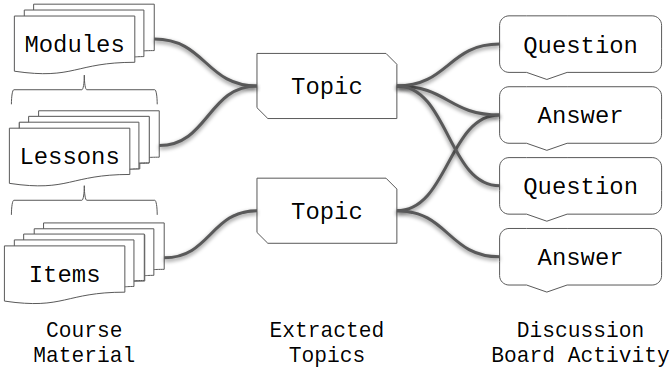
\includegraphics[width=\columnwidth]{fig/data_model.png}
    \caption{Course material consists of modules, lessons, and items. Topics infer discussion board activity. Topics have a many-to-many relationship to course material.}
    \label{fig:data_model}
\end{figure}

\begin{figure}
    \centering
    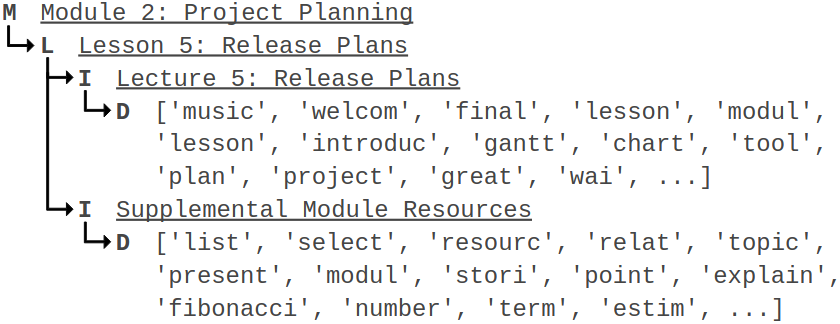
\includegraphics[width=\columnwidth]{fig/sample_doc.png}
    \caption{Two documents (D) from "Agile Planning for Software Products" with corresponding labels (M, L, I).}
    \label{fig:sample_doc}
\end{figure}

\subsection{Topic Analysis Approaches}
Topics were extracted from the course content material using unsupervised and supervised LDA.
New models were trained for each course.
We used the \texttt{gensim@3.7.1} implementation of LDA, Hierarchical Dirichlet Process LDA (HDP-LDA) and Author-Topic model~\cite{rehurek_lrec}.
To form our unsupervised set of topics, we used both LDA and HDP-LDA.
All LDA parameters were set as the library provided defaults ($\text{num\_topics}=100$, $\alpha=0.01$, $\beta=0.001$).
HDP-LDA addresses one shortcoming of traditional LDA by using a Dirichlet process to capture the number of topics, rather than defining the number of topics a priori~\cite{wang2011online}.
We ran HDP-LDA with the default configuration provided by the library ($\kappa=1$, $\tau=64$, $K=15$, $T=150$, $\alpha=1$, $\gamma=1$, $\eta=0.01$).

The Author-Topic model, an extension of base LDA, was introduced by \citeauthor{rosen2004author} to correlate documents with authorship information to provide more details on the subject knowledge of the given author~\cite{rosen2004author}.
The Author component of the Author-Topic model is classically represented by labeling an existing corpus of documents with the author(s) of the document.
However, we modified the standard usage and replaced Author with \texttt{modules}, \texttt{lessons}, and \texttt{items}.
The underlying assumption was course subject knowledge labeled by subject headings could be analogous to course content labeled by the content author.
The parameter choices for the Author-Topic model was left as the library provided defaults ($\text{num\_topics}=100$, $\alpha=0,01$, $\beta=0.001$).

Additional topic analysis using Labeled LDA was run.
Unlike Author-Topic models, Labeled LDA outputs topics constrained to the labels defined in the corpus~\cite{ramage2009labeled}.
Classical applications of Labeled LDA are analyzing tagged blog entries, where a given blog may have multiple associated tags.
We extend an existing implementation of Labeled LDA found on GitHub, with slight modification for topic inference without training~\footnote{Labeled LDA in Python.
    %\url{https://github.com/fann1993814/llda}
    %\url{https://github.com/shuyo/iir}
    URL DOUBLE BLIND HIDDEN}.
Our parameter choices for Labeled LDA are $\alpha=0.01$, $\text{beta}=0.001$, with 50 iterations.
The differences between the four studied models are defined in Table~\ref{tab:topic_models}. We use the \texttt{module}, \texttt{lesson}, and \texttt{item} names as labels for our Author-Topic and Labeled LDA approaches.

\begin{table}
    \centering
    \begin{tabularx}{\columnwidth}{@{}lccc@{}}
    \toprule
    Topic Model & Labels & Topic Characteristic & Num. Topics \\
    \midrule
    LDA & \texttt{False} & bounded, latent & set 100 \\
    HDP-LDA & \texttt{False} & unbounded, latent  & capped 150 \\
    Author-Topic & \texttt{True} & distributed over labels & set 100 \\
    Labeled LDA & \texttt{True} & restricted to labels & Num. labels \\
    \bottomrule
    \end{tabularx}
    \caption{Comparison of the four different topic analysis models used in our study.}
    \label{tab:topic_models}
\end{table}

\subsection{Relating Topics to Discussion Activity}
To derive a relationship between discussion forum activity and the course material, we used our trained topic models to infer topic distribution of the discussion form posts.
We inferred the relationship between the word distribution within the discussion post and the word distribution within the topic.
We applied the same pre-processing step from the course material on the discussion forum activity. We removed tags, punctuation, consecutive white-space, numbers, stop words, and words less than three characters in length before stemming all remaining words to their root word.

LDA inference takes as input a set of documents and estimates the topic weight distribution for each document.
Because LDA does not modify the existing model and no learning occurs, we performed inference using only the subset of words in the discussion entity that have appeared in our course material vocabulary.
These discussion questions and answers were related to pre-existing topics extracted from the course material.

\begin{equation}
    \text{Cosine Distance} = 1 - \frac {\pmb A \cdot \pmb B}{||\pmb A||_2 ||\pmb B||_2}
    \label{eq:cos_distance}
\end{equation}

% AH: wrong order, say the task and then the tool for the task
% do you mean the document-topic vector for the document or the
% whole vector % addressed.
% order? what's teh point do you want to say a discussion post is topical?
If a discussion post has similar topics to a given lecture, we want to suggest that lecture as a likely candidate for the post.
Specifically, the document-topic vector of the discussion post is compared with the document-topic vector of the course item.
To determine topic similarity, we used cosine distance as defined in Equation~\ref{eq:cos_distance}.
The cosine distance function returns a floating value between 0 and 1. As the cosine distance approaches 1, the two elements are more distinct. The two elements are more similar as the cosine distance approaches 0.

% you're using cosine distance as a score for the best topic
% or the best document? What's the point?
% or are you going back to documents that the topic originated?
% what's the actual score here. The topic cosines or the document cosines or what

\subsection{Evaluating Discussion Classification}

% explain it better
% what is being returned? documents or topics
% how are they ranked: cosine distance
% are they in order: cosine distance

To determine the effectiveness of our models in tracing discussion forum text back to the underlying course content, we randomly sampled from the discussion activity and manually assigned the discussion to the underlying course item.
Only the primary author labeled the discussion posts.
Labelling the discussion posts was challenging as there were many discussions that did not have a clear mapping to one course item.
Discussion posts that were blatantly off topic were excluded from evaluation, using the researcher's judgment.
We evaluated our models on 100 manually classified posts for each of the 7 courses.
% AH: how do you know it's the underlying course item? % addressed

\begin{equation}
    \text{Mean Reciprocal Rank} = \frac{1}{|Q|} \sum^{|Q|}_{i=1}\frac{1}{\text{rank}_i}
    \label{eq:mrr}
\end{equation}

We evaluated the model provided forum post ordering with our manually labeled discussion data using mean reciprocal rank (MRR), as shown in Equation~\ref{eq:mrr}.
Given a sample number of queries $Q$, we return the multiplicative inverse of the rank for the correct answer.
For example, if the model ranked a discussion question with our value in the first place, the MRR would be $1$.
Second and third place would be $\frac{1}{2}$ and $\frac{1}{3}$ respectively.

\section{Results}
The calculated MRRs derived from our analyzed courses are shown in Table~\ref{tab:result_mrrs}. The baseline TF-IDF model outperforms topic models in all courses except for "Introduction to Software Product Management". The least effective model for discussion forum traceability was the Author-Topic model, as it had the lowest MRR for four of the five courses. 

\begin{figure}
    \centering
    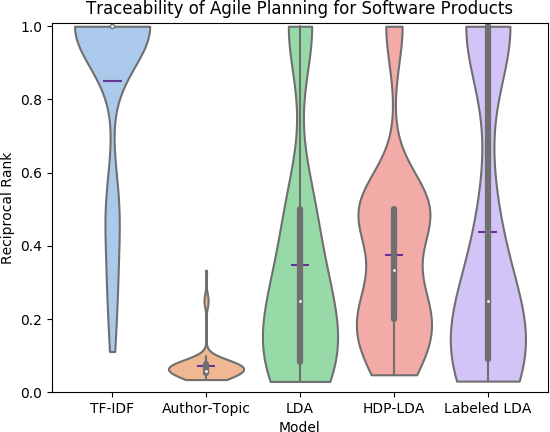
\includegraphics[width=\columnwidth]{fig/agile-planning.png}
    \caption{Reciprocal rank violin plot for "Agile Planning for Software Products". Horizontal line indicates model MRR.}
    \label{fig:my_label}
\end{figure}

\begin{table*}[t]
    \centering
\noindent\begin{tabular}{r*{5}{|p{0.2\columnwidth}}|}
 \multicolumn{1}{c}{} & \multicolumn{1}{c}{TF-IDF} & \multicolumn{1}{c}{Author-Topic} 
  & \multicolumn{1}{c}{LDA} & \multicolumn{1}{c}{HDP-LDA} & \multicolumn{1}{c}{Labeled LDA} \\ \hhline{~*5{|-}|}
 Agile Planning for Software Products           & \bf 0.851 & 0.072 & 0.347 & 0.374 & 0.439 \\ \hhline{~*5{|-}|}
 Client Needs and Software Requirements         & \bf 0.650 & 0.351 & 0.169 & 0.456 & 0.262 \\ \hhline{~*5{|-}|} 
 Design Patterns                                & \bf 0.661 & 0.062 & 0.295 & 0.168 & 0.327 \\ \hhline{~*5{|-}|}
 Introduction to Software Product Management    & 0.209 & 0.052 & 0.100 & 0.206 & \bf 0.238 \\ \hhline{~*5{|-}|}
 Object Oriented Design                         & \bf 0.925 & 0.094 & 0.462 & 0.272 & 0.436 \\ \hhline{~*5{|-}|}
\end{tabular}\par\bigskip
    \caption{Mean reciprocal ranks for the baseline and four topic models on our five courses. Values closer to 1 are better.}
    \label{tab:result_mrrs}
\end{table*}

\section{Discussion}
TODO

\section{Threats to Validty}
TODO

\section{Future Work}
One limitation of our current approach is the inability to handle off topic discussions.
Many discussions were either unrelated to the course, or were too general to be mapped appropriately to a single course item.
Future relevant work includes investigating how to best model "Off-Topic" discussion posts, and how to accommodate course material relevance granularity.

We provide the source code used to perform this experiment in the intent that replication studies of this work can be performed on other MOOCs~\footnote{Source code for research experiment.
    % link to github
    URL DOUBLE BLIND HIDDEN}.
Our study focuses entirely on computer science and software engineering courses.
Another potential replication study could measure if discussion topicality matches course material across courses in Arts and Humanities, Business, Mathematics, Science, and other varying domains.

\section{Conclusion}
TODO

\bibliographystyle{ACM-Reference-Format}
\bibliography{references}

\end{document}
